\section{Results}\label{sec:results}
\subsection{Surface Density Projections}\label{ssec:projections}
Before dissecting the simulated galaxies in detail, we first take a look at the surface density projections of the gas and stars in the central region, situated on the central galaxy. This is shown in Figure~\ref{fig:projections}. In each grouping of four, the bottom and top rows show the face-on and edge-on views, respectively. The left and right columns show the gas and stellar surface density. Each panel is oriented with respect to the stellar angular momentum of the final snapshot ($t=8\,\Gyr$). The angular momentum is computed using all star particles within the half-mass radius.

\begin{figure*}
  \centering
  \includegraphics[width=\textwidth]{surfdens.pdf}
  \caption{The surface density projections of the gas and stars over time of the idealized merger simulation with $R_0=142\,\kpc$, $V_0=116\,\kms$, and $\eta=0.4$ (i.e., the ``bimodal'' simulation). Every panel is oriented with respect to the final ($t=8\,\Gyr$) snapshot. In each grouping of four, the lower and upper rows show the face-on and edge-on projections, respectively. The left and right columns show the gas and stellar surface densities, respectively. The side-length of each panel is $30\,\kpc$, and the image is a projection through a box with the same side-length. \red{Need to fix spacing between panels and add scale bar.}}
  \label{fig:projections}
\end{figure*}

\subsection{Abundance Distribution}\label{ssec:abundplane}
In Figure~\ref{fig:fig1}, briefly discussed in Section~\ref{sec:intro}, we show the abundance distribution of the Milky Way as well as two of our idealized merger simulations in the upper panels. A number of our idealized simulations exhibit either a bimodal or unimodal abundance distribution, and so we have selected two representative examples. The simulation labeled bimodal had orbital parameters of $R_0=142\,\kpc$, $V_0=116\,\kms$, and $\eta=0.4$. The unimodal simulation is identical, except that $R_0=129\,\kpc$.

There are, of course, differences between the bimodal simulation and the Milky Way. First, the scaling in \MgFe{} is different -- in the simulation, the low-$\alpha$ sequence lies at $\sim0.2$, while in the Milky Way it is at about $\MgFe\sim0$. Second, in the Milky Way the high-$\alpha$ sequence neatly joins the low-$\alpha$ sequence at $\FeH\sim0$, while in the simulation the two actually diverge more at higher \FeH{}. Finally, at high \FeH{} the distribution bends upwards while in the simulation it bends downwards.

Finally, in the lower panels of Figure~\ref{fig:fig1}, we show the distributions of \MgFe{} at different fixed \FeH{}. The (blue, orange, red, green) lines show the \MgFe{} distribution at a \FeH{} of ($-0.5$, $-0.375$, $-0.25$, $0.25$), in bins of width $0.05\,\dex$. The distributions of \MgFe{} are offset (but not rescaled) so that they do not overlap. Here, the bimodality seen in the Milky Way is quite striking at lower metallicities. The peaks are well-separated, by $\sim0.2\,\dex$. In the bimodal simulation, the distribution is still clearly bimodal, but the peaks are less well-separated, by $\sim0.1\,\dex$. In the unimodal simulation, the distributions are clearly unimodal, with the hint of some structure in the $\FeH=0.25\,\dex$ bin.

\subsection{Build up of the Abundance Plane}\label{ssec:abundplane_build}
Next, we examine the build up of the abundance plane. First, in Figure~\ref{fig:before_after}, we show the abundance plane at various points along the merger. We have divided the history of the merger into ``before'' ($t < 1.5\,\Gyr$), ``during'' ($1.5\,\Gyr < t < 2.5\,\Gyr$), and ``after'' ($t > 2.5\,\Gyr$). These times have been chosen somewhat by the orbital history and somewhat by visually inspecting the simulation, and so these deliniations are, to an extent, arbitrary. Nonetheless, it is clear that the high-$\alpha$ sequence forms before and during the merger (middle panels), and that the low-$\alpha$ sequence forms after the merger (right panel). We show a dashed line given by $-0.1\FeH + 0.31$, which is a crude way of separating the high- and low-$\alpha$ sequence.

It is informative to examine the star formation history (SFH) split into the high- and low-$\alpha$ sequences, shown in Figure~\ref{fig:before_after_sfh}. The high- and low-$\alpha$ sequences (blue and orange) are defined as the star particles lying above and below the dashed line in Figure~\ref{fig:before_after}, respectively. We show this only in a narrow bin of width $0.1\,\dex$ at $\FeH\sim0$. One can see a very clear separation in time between the high- and low-$\alpha$ sequences, with the high-$\alpha$ sequence forming before the low-$\alpha$ sequence.\footnote{There is a small amount of low-$\alpha$ formation at the very end of the high-$\alpha$ sequence, but this can be understood as simply an inadequacy in our simple way of separating the two sequences.} Furthermore, there is a brief period of $\sim300\,\Myr$ between the two sequences where no stars have formed.

It can also be shown that the exact timing of this quiescent period is metallicity-dependent. We show the same SFH, but at varying bins in \FeH{} of $-0.5$, $-0.25$, and $0$ (blue, orange, and red, respectively). For clarity, we do not separate the SFHs by the high- and low-$\alpha$ sequences, but have verified that the same demarcation arises as in Figure~\ref{fig:before_after_sfh}. Here, we can see that at $\FeH=-0.5$ the quiescent period begins $\sim250\,\Myr$ earlier than at $\FeH=0$.

\subsection{\alphaFe{} Behavior Associated with Quiescence}
Given the sequence of events presented in Section~\ref{ssec:abundplane_build}, it is natural to suspect that the quiescent phase in Figure~\ref{fig:before_after_sfh} is responsible for the bimodal structure in Figure~\ref{fig:before_after}. We now examine this possibility more closely.

In Figure~\ref{fig:SFR_alpha}, we show the SFR (blue lines) of each of the bimodal and unimodal galaxies (left and right panels, respectively) as well as the median \MgFe{} of the gas (orange lines) in a bin centered on $\FeH{}=-0.1$ with width $0.02\,\dex$. The SFR is shown for the entire galaxy ($r<15\,\kpc$) while the median \MgFe{} is shown for $2\,\kpc<r<5\,\kpc$.\footnote{The solar neighborhood-like selection of stars mostly selects stars at $2\,\kpc<r<5\,\kpc$. We choose to plot the median \MgFe{} of the gas at these radii, since it is that gas which is forming stars that ends up in our sample. On the other hand, we choose to show the SFR for the entire galaxy, as the enrichment from that star formation affects the entire galaxy.} 

The merger appears to induce a starburst, where the SFR rises from $\sim3.5\,\Msunyr$ at $\sim1\Gyr$ to a peak of $\sim12\,\Msunyr$ at $\sim2\,\Gyr$. This starburst is then followed by a quiescent period, with a depth of $\sim1\,\Msunyr$ and a duration of $\sim500\,\Myr$. The dip in SFR is not as pronounced as it was when we plotted the SFH at a particular iron (Figure~\ref{fig:before_after_sfh}). This quiescent period is associated with a sudden drop in \MgFe{}. In $\sim250\,\Myr$, \MgFe{} drops from $\sim0.35$ to $\sim0.2\,\dex$. Once the SFR recovers $\sim500\,\Myr$ later, \MgFe{} again rises, but only to $\sim0.28\,\dex$.

This behavior is present in the unimodal simulation (right panel) -- it does not display a period of suppressed star formation, and there is no associated drop in \MgFe{}. It does still have a period of enhanced star formation, but this is actually coincident with an enhancement in \MgFe{}. This sequence of events is further emphasized in Figure~\ref{fig:alpha_vs_tform}, which shows a transparent scatter plot of \MgFe{} as a function of formation time. In the bimodal simulation, there is a clear gap in \MgFe{} during the period of quiescence followed by the brief formation of $\alpha$-deficient stars. In the unimodal simulation, on the other hand, there is no gap and the brief formation of $\alpha$-enhanced stars.

\subsection{Cause of Quiescence}\label{ssec:cause_qui}
The exact cause of quiescence in our simulation is not the main focus of our work. However, it appears to arise as a result of AGN activity triggered by the merger. We present some evidence of this in Appendix~\ref{app:cause_qui}.

\begin{figure*}
  \centering
  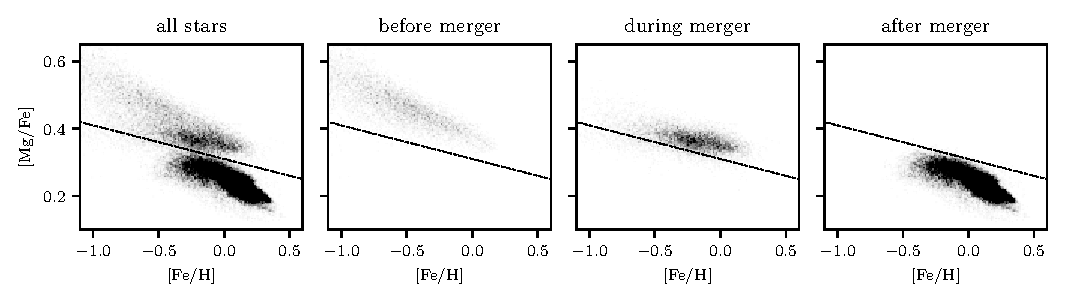
\includegraphics[width=\textwidth]{before_after.pdf}
  \caption{\textbf{The high-$\alpha$ sequence forms before the merger, the low-$\alpha$ sequence forms after the merger.} This plot shows the sequence of events leading to the build-up of the low- and high-$\alpha$ sequences for our fiducial bimodal simulation. We have separated the high- and low-$\alpha$ sequences by a dashed line at $-0.1\FeH + 0.31$, which was chosen by eye to lie in the trough. The left panel shows all star particles in our solar neighborhood cut. The middle left panel shows the star particles that form before the merger ($\tform < 1.5\,\Gyr$), which form a weak sequence of star particles at the lowest \FeH and highest \MgFe. The middle right panel shows the star particles that form during the merger ($1.5\,\Gyr < \tform < 2.5\,\Gyr$). These star particless form the portion of the high-$\alpha$ sequence closest to the trough, and the density of star particless is higher than those that form before. The middle right panel shows the star particles which form after the merger ($\tform > 2.5\,\Gyr$). These star particles form almost entirely below the trough.}
  \label{fig:before_after}
\end{figure*}

\begin{figure}
  \centering
  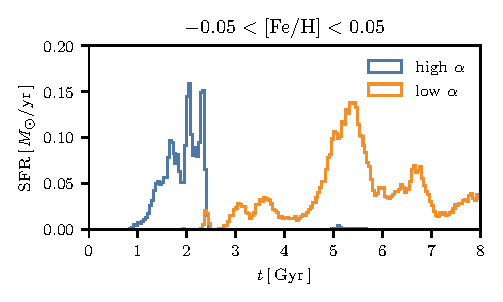
\includegraphics[width=\columnwidth]{before_after_sfh.pdf}
  \caption{\textbf{At fixed metallicity, the low- and high-$\alpha$ sequence are cleanly separated in time, with an intervening quiescent period.} Here we show the star formation history of the high- and low-$\alpha$ sequences. The blue (low-$\alpha$) and orange (high-$\alpha$) histograms correspond to the dashed line cut made in the \MgFe-\FeH plane in Figure~\ref{fig:before_after}, at a fixed metallicity of $\FeH\sim0$. One can see that there is a nearly perfect separation in time between the formation of the high-$\alpha$ and low-$\alpha$ sequence, except for a brief overlap which can be attributed to the inadequacy of the linear cut model of the two sequences. Separating the formation periods lies a quiescent period with a duration of $\sim300\,\Myr$. \red{make sfr per dex}.}
  \label{fig:before_after_sfh}
\end{figure}

\begin{figure}
  \centering
  \includegraphics[width=\columnwidth]{before_after_sfh_by_iron.pdf}
  \caption{\textbf{The timing of the quiescent period which divides the high- and low-$\alpha$ sequences is metallicity dependent.} The star formation history of stars at various fixed metallicities ($\FeH\sim0$, $-0.25$, and $-0.5\,\textrm{dex}$). As in Figure~\ref{fig:before_after_sfh}, there is a quiescent period period which separates the formation of the low- and high-$\alpha$ sequence \red{maybe a better way to show this?}. However, one can see that the timing of the quiescent period is metallicity-dependent. It occurs earlier at lower metallicity, by $\sim300\,\Myr$ for the metallicities shown in this plot. \red{make sfr per dex}.}
  \label{fig:before_after_sfh_by_iron}
\end{figure}

\begin{figure*}
  \centering
  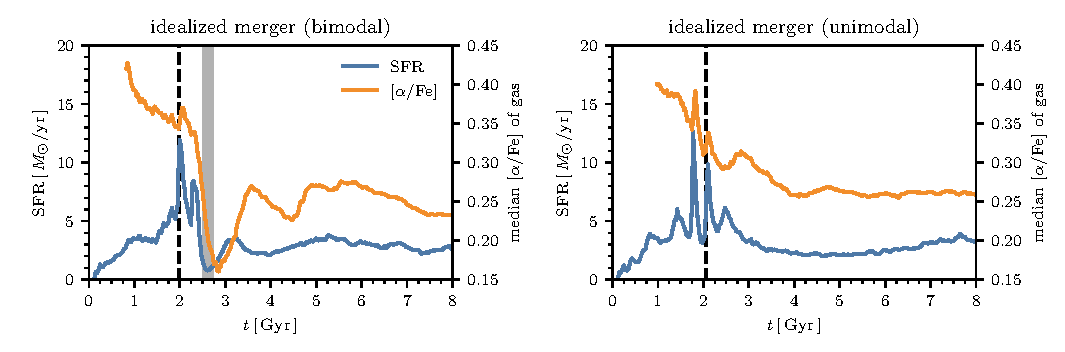
\includegraphics[width=\textwidth]{SFR_alpha.pdf}
  \caption{\textbf{A global suppression of star formation is associcated with a decrease in \MgFe{}, which is seen in the bimodal simulation but not in the unimodal simulation.} Here, we show both the SFR of the central galaxy ($r<15\,\kpc$) and the median \MgFe{} for gas at $2\,\kpc<r<5\,\kpc$ at a fixed \FeH{} bin centered on $-0.2$ with width $0.02\,\dex$. The left panel shows the bimodal simulation while the right panel shows the unimodal simulation. The time of the merger (i.e., the second pericenter) is indicated by the vertical dashed line. In the bimodal simulation, the star formation is suppressed after the merger. This suppression of star formation is associated with a sudden drop in the median \MgFe{} of the gas. Neither the suppression of star formation nor the drop in \MgFe{} are seen in the unimodal simulation.}
  \label{fig:SFR_alpha}
\end{figure*}

\begin{figure}
  \centering
  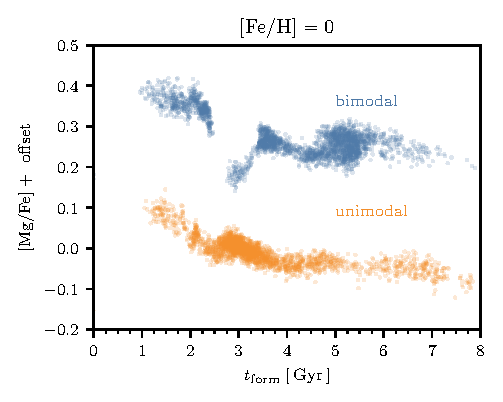
\includegraphics[width=\columnwidth]{alpha_vs_tform.pdf}
  \caption{The formation times and \MgFe{} values of star particles in the bimodal (blue) and unimodal (orange) simulations. In the bimodal simulation, a gap in stellar ages is briefly followed by the formation of $\alpha$-deficient star particles. In the unimodal simulation, no gap is present and there is briefly the formation of $\alpha$-enhanced star particles at the same time. The \MgFe{} values of the unimodal simulation have been offset by $-0.3$ for clarity.}
  \label{fig:alpha_vs_tform}
\end{figure}
